\documentclass[a4paper,12pt]{article}
\usepackage{amsmath,amssymb,amsfonts,amsthm}
\usepackage{tikz}
\usepackage [utf8x] {inputenc}
\usepackage [T2A] {fontenc} 
\usepackage[russian]{babel}
\usepackage{cmap, upgreek}
\usepackage{textcomp} 

% Так ссылки в PDF будут активны
\usepackage[unicode]{hyperref}

% вы сможете вставлять картинки командой \includegraphics[width=0.7\textwidth]{ИМЯ ФАЙЛА}
% получается подключать, как минимум, файлы .pdf, .jpg, .png.
\usepackage{graphicx}
% Если вы хотите явно указать поля:
\usepackage[margin=1in]{geometry}
% Или если вы хотите задать поля менее явно (чем больше DIV, тем больше места под текст):
% \usepackage[DIV=10]{typearea}

\usepackage{fancyhdr}

\newcommand{\bbR}{\mathbb R}%теперь вместо длинной команды \mathbb R (множество вещественных чисел) можно писать короткую запись \bbR. Вместо \bbR вы можете вписать любую строчку букв, которая начинается с '\'.
\newcommand{\eps}{\varepsilon}
\newcommand{\bbN}{\mathbb N}
\newcommand{\dif}{\mathrm{d}}

\newtheorem{Def}{Определение}


\pagestyle{fancy}
\makeatletter % сделать "@" "буквой", а не "спецсимволом" - можно использовать "служебные" команды, содержащие @ в названии
\fancyhead[L]{\footnotesize Электричество и магнетизм}%Это будет написано вверху страницы слева
\fancyhead[R]{\footnotesize ФМХФ МФТИ}
\fancyfoot[L]{\footnotesize \@author}%имя автора будет написано внизу страницы слева
\fancyfoot[R]{\thepage}%номер страницы —- внизу справа
\fancyfoot[C]{}%по центру внизу страницы пусто

\renewcommand{\maketitle}{%
	\noindent{\bfseries\scshape\large\@title\ \mdseries\upshape}\par
	\noindent {\large\itshape\@author}
	\vskip 2ex}
\makeatother
\def\dd#1#2{\frac{\partial#1}{\partial#2}}


\title{3.6.1 \\ Спектральный анализ электрических сигналовюю}
\author{Егор Берсенев} 
\date{15 апреля 2016 г.}

\begin{document}
	\maketitle
	\section{Цель работы}
		 Изучение спектрального состава периодических электрических сигналов.
	\section{Оборудование}
		Анализатор спектра, генератор прямоугольных сигналов, генератор сигналов специальной формы, осциллограф.
	\section{Теоретическая часть}
		В работе изучается спектральный состав различных типов сигналов: последовательности прямоугольных импульсов, последовательности цугов и амплитудно-модулированных колебаний.
		\subsection{Периодическая последовательность прямоугольных импульсов}
			Пусть амплитуда $V_0$, длительностью $\tau$, частотой повторения $\Omega_1 = \frac{2\pi}{T}$, где $T$ --- период повторения импульсов.
			Найдем среднее значение амплитуды:
			$$
			\left<V\right> = \frac{a_0}{2} = \frac{A_0}{2} = \frac{1}{T}\int_{-r/2}^{r/2}V_0\dif t = \frac{\tau}{T}V_0
			$$
			Коэффициенты при косинусах равны:
			$$
			a_n = \frac{2}{T}\int_{-r/2}^{r/2}V_0\cos\left(n\upomega_1t\right)\dif t = 2V_0\frac{\tau}{T}\frac{\sin\left(n\Omega_1\tau/2\right)}{n\Omega_1\tau/2}\simeq\frac{\sin x}{x}
			$$
		\subsection{Периодическая последовательность цугов}
			Рассмотрим цуги гармонического колебания $V_0\cos\left(\omega_0t\right)$ с длительностью цуга $\tau$ и периодом повторения $T$.
			Коэффициент при n-й гармонике равен:
			$$
			a_n = \frac{2}{T}\int_{-r/2}^{r/2}V_0\cos\left(\omega_0t\right)\cdot\cos\left(n\Omega_1t\right)\dif t = V_0\frac{\tau}{T}\left(\frac{\sin\left[\left(\omega_0 - n\Omega_1\right)\frac{r}{2}\right]}{\left(\omega_0 - n\Omega_1\right)\frac{r}{2}} + \frac{\sin\left[\left(\omega_0 + n\Omega_1\right)\frac{r}{2}\right]}{\left(\omega_0 + n\Omega_1\right)\frac{r}{2}}\right)			
			$$
			
		\subsection{Амплитудно-модулированные колебания}
		Рассмотрим гармонические колебания высокой частоты $\omega_0$, амплитуда которых меняется с частотой $\Omega$, $\left(\Omega \ll \omega\right)$. 
		$$
		f(t) = A_0\left[1+m\cos\Omega t\right]\cos\omega t
		$$
		m называется глубиной модуляции. Простым тригонометрическим преобразованием найдем спектр таких колебаний:
		$$
		f(t) = A_0\cos\omega_0t + \frac{A_0m}{2}\cos\left(\Omega+\omega_0\right)t+\frac{A_0m}{2}\cos\left(w_0-\Omega\right)t
		$$
	\section{Ход работы}
		\subsection{Периодическая последовательность прямоугольных импульсов}
		Соберем экспериментальную установку:
		
		\includegraphics[width = 0.7\linewidth]{scheme1}
		
		Спектры:
		
		\begin{figure}[h]
			\begin{minipage}[h]{0.32\linewidth}
				\centering
				\includegraphics[width=0.9\linewidth]{pic1} \\ 1кГц, 25мкс
			\end{minipage}
			\hfill
			\begin{minipage}[h]{0.32\linewidth}
				\centering
				\includegraphics[width=0.9\linewidth]{pic2} \\ 1кГц, 50мкс
			\end{minipage}
			\hfill
			\begin{minipage}[h]{0.32\linewidth}
				\centering
				\includegraphics[width=0.9\linewidth]{pic3} \\ 2кГц, 25мкс
			\end{minipage}
		\end{figure}
		
		Проведем измерения:
		
		\begin{table}[h]
			\centering
			\caption{Прямоугольные импульсы}
			\label{my-label}
			\begin{tabular}{|l|l|l|l|l|l|l|}
				\hline
				$\tau$, мкс      & 25 & 50 & 100 & 125 & 150 & 170 \\ \hline
				x, дел          & 6  & 4  & 2   & 1.6 & 0.8 & 0.4 \\ \hline
				$\Delta\nu$, кГц & 40 & 20 & 10  & 8   & 4   & 2   \\ \hline
				$1/\tau$, кГц  & 40 & 20 & 10  & 8   & 6.7 & 5.9 \\ \hline
			\end{tabular}
		\end{table}
		
		Огибающие: 
		
		\begin{figure}[h]
			\begin{minipage}[h]{0.49\linewidth}
				\centering
				\includegraphics[width=0.9\linewidth]{pic4} \\ 1кГц, 50мкс
			\end{minipage}
			\hfill
			\begin{minipage}[h]{0.49\linewidth}
				\centering
				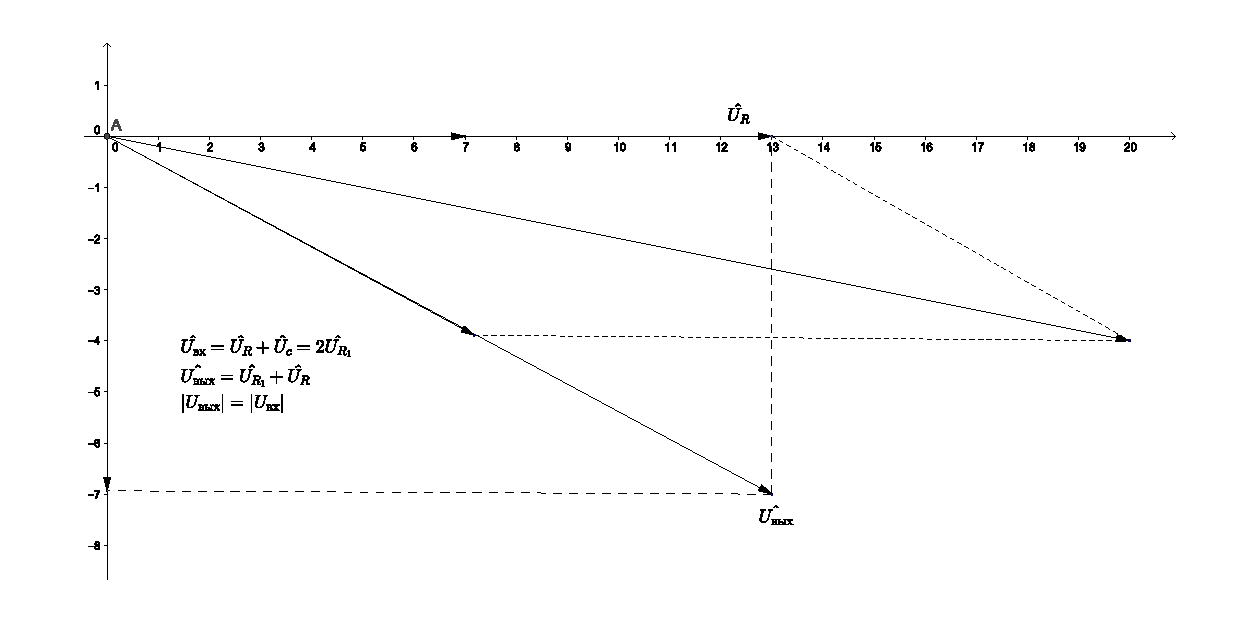
\includegraphics[width=0.9\linewidth]{pic5} \\ 1кГц, 100мкс
			\end{minipage}
			\hfill
		\end{figure}
		
		Построим график:
		
		\includegraphics[width = 0.7\linewidth]{graphA}
		
		Отсюда убеждаемся, что соотношение неопределенностей справедливо.
		
		\subsection{Исследование спектра периодической последовательности цугов гармонических колебаний}
		Соберем экспериментальную установку: 
		
		\includegraphics[width = 0.7\linewidth]{scheme2}
		
		Установим несущую частоту $\nu_0 = 25$ кГц и получим спектры:
		
		\begin{figure}[h!]
			\begin{minipage}[h]{0.49\linewidth}
				\centering
				\includegraphics[width=0.9\linewidth]{pic6} \\ 1кГц, 50мкс, $\nu_0 = 25$ кГц
			\end{minipage}
			\hfill
			\begin{minipage}[h]{0.49\linewidth}
				\centering
				\includegraphics[width=0.9\linewidth]{pic7} \\ 1кГц, 50мкс $\nu_0 = 10$ кГц
			\end{minipage}
		\end{figure}
		
		\begin{figure}[h!]
			\begin{minipage}[h]{0.49\linewidth}
				\centering
				\includegraphics[width=0.9\linewidth]{pic8} \\ 1кГц, 100мкс, $\nu_0 = 25$ кГц
			\end{minipage}
			\hfill
			\begin{minipage}[h]{0.49\linewidth}
				\centering
				\includegraphics[width=0.9\linewidth]{pic9} \\ 1кГц, 50мкс $\nu_0 = 40$ кГц
			\end{minipage}
		\end{figure}
		
		\newpage
		Сделаем измерения:
		
		\begin{table}[h!]
			\begin{tabular}{|l|l|l|l|l|l|l|l|l|}
				\hline
				$f_\text{повт}$, кГц           & 1   & 2 & 3   & 4 & 5    & 6 & 7   & 8   \\ \hline
				x, дел           & 0.5 & 1 & 1.5 & 2 & 2.27 & 3 & 3.8 & 4.1 \\ \hline
				$\Delta\nu$, кГц  & 1   & 2 & 3   & 4 & 5.5  & 6 & 7.6 & 8.2 \\ \hline
			\end{tabular}
			
			
		\end{table}
		
		Построим график:
		
		\includegraphics[width = 0.7\linewidth]{graphB}
		
		Отсюда также убеждаемся в справедливости соотношения неопределенностей.
		
		\subsection{Исследование спектра амплтиудно-модулированных гармонических колебаний}
		
		Соберем установку:
		
		\includegraphics[width = 0.7\linewidth]{scheme3}
		
		Сделаем измерения:
		
		\begin{table}[h]
			\begin{tabular}{|l|l|l|l|l|l|}
				\hline
				$2A_{min}$                           & 0    & 0.04 & 0.04 & 0    & 0.06 \\ \hline
				$2A_{max}$                           & 0.24 & 0.20 & 0.16 & 0.44 & 0.14 \\ \hline
				$a_\text{бок}$                     & 2.17 & 1.33 & 1    & 2.50 & 0.80 \\ \hline
				$a_\text{осн}$                     & 4.33 & 4.33 & 4.33 & 4.00 & 4.00 \\ \hline
				$m$                                  & 1    & 0.67 & 0.6  & 1    & 0.4  \\ \hline
				$a_\text{бок}/a_\text{осн}$ & 0.5  & 0.31 & 0.23 & 0.63 & 0.2  \\ \hline
			\end{tabular}
		\end{table}
		
		Построим график:
		
		\includegraphics[width = 0.7\linewidth]{graphC}
		
	\section{Вывод}
		Фурье-анализ позволяет получать спектр периодических электрических сигналов, что дает возможность исследовать большое количество свойств
		
\end{document}


